\documentclass[a4paper,11pt]{article}
\usepackage[utf8]{inputenc}
\usepackage[T1]{fontenc}
\usepackage[top=1.5cm, bottom=1.5cm, left=1.5cm, right=1.5cm]{geometry}

\title{Syntax driven source code merge}
\author{Guillaume Bertholon}

\usepackage{listings-rust}
\lstset{
  language=Rust,
  breaklines=true,
  extendedchars=true,
  captionpos=b,
  style=boxed,
  escapechar=@,
  % We want to disable any syntax coloring to focus on awareness colors
  stringstyle=,
  keywordstyle=,% reserved keywords
  keywordstyle=[2],% traits
  keywordstyle=[3],% primitive types
  keywordstyle=[4],% type and value constructors
  keywordstyle=[5],% macros
}

\usepackage{tikz}
\usetikzlibrary{calc}
\usetikzlibrary{positioning}
\usetikzlibrary{shapes.geometric}
\tikzstyle{varnode} = [draw, circle, text height=1.5ex, text depth=.25ex, align=center]
\tikzstyle{mvnode} = [draw, regular polygon, regular polygon sides=3, text height=1.5ex, text depth=.25ex, align=center, inner sep=2]
\tikzstyle{changenode} = [draw, rectangle, scale=0.8]
\tikzstyle{condnode} = [draw, diamond]
\tikzstyle{conflict} = [red, fill=red!10]
\tikzstyle{colorA} = [fill=blue!30]
\tikzstyle{colorB} = [fill=orange!40]
\tikzstyle{colorDel} = [fill=red!20]
\tikzstyle{colorIns} = [fill=olive!20]

\usepackage{bussproofs}
\usepackage{amsmath}
\usepackage{soul}
\usepackage{amssymb}
\usepackage{stackengine}
\renewcommand\vec[1]{\overrightarrow{#1}}
\newcommand\typsep{\mathrel{|}}
\newcommand\typ[1]{\mathrm{#1}}
\newcommand\typarg[2]{\typ{#1}\langle#2\rangle}
\newenvironment{typgrammar}{
\par\vspace{0.5em}\centering
$\displaystyle\begin{aligned}}{\end{aligned}
$\par\vspace{0.5em}}
\newcommand\synnode[2]{#1[#2]}
\newcommand\syntoken[1]{``#1"}
\newcommand\synfield[2]{#1.#2}
\newcommand\merge{\mathbin{\Join}}
\newcommand\del[1]{\text{\st{$#1$}}}
\newcommand\ins[1]{\text{\ul{$#1$}}}
\newcommand\id{\square}
\newcommand\change[2]{\del{#1} \rightarrow \ins{#2}}
\newcommand\keyword[1]{\mathbf{#1}}
\DeclareMathOperator\InsConflict{Ins!}
\DeclareMathOperator\DelConflict{Del!}
\DeclareMathOperator\OrdConflict{Ord!}
\DeclareMathOperator\MvConflict{Mv!}
\DeclareMathOperator\dom{dom}
\newcommand\rewritten{\rightsquigarrow}
\allowdisplaybreaks

\usepackage{hyperref}
\hypersetup{hidelinks}

\usepackage[title]{appendix}
\usepackage[section]{placeins}

\begin{document}

\maketitle

\newcommand{\TODO}[1]{\textcolor{red}{$\langle$ TODO:} #1 \textcolor{red}{$\rangle$}}

%%%%%%%%%%%%%%%%%%%%%%%%%%%%%%%%%%%%%%%%%%%%%%%%%%%%%%%%%%%%%%%%
%% Syntax of trees

\newcommand{\aNode}{\ensuremath{\mathsf{node}}}
\newcommand{\aField}{\ensuremath{\mathsf{field}}}
\newcommand{\aAtom}{\ensuremath{\mathsf{atom}}}
\newcommand{\aTree}{\ensuremath{\mathsf{t}}}
\newcommand{\many}[1]{\ensuremath{\overrightarrow{#1}}}

\newcommand{\defNode}[2]{\ensuremath{#1 \{ #2 \}}}
\newcommand{\defField}[2]{\ensuremath{#1 : #2}}

%%%%%%%%%%%%%%%%%%%%%%%%%%%%%%%%%%%%%%%%%%%%%%%%%%%%%%%%%%%%%%%%


\section{Computing difference between syntax trees}

\paragraph{Generic syntax tree}
Before starting we want to define a unified syntax tree type that can
represent any parsed file in any language. \TODO{Rather: ``generic''
  datastructure to represent parse trees. Key intuition: use tagged
  sum (thanks to \defNode{-}{=}) of named products (thanks to
  \defField{-}{=}).}

For that we will use a tree with labelled
nodes and arbitrary list of possibly labeled children, and take the convention
that leaves represent tokens in the input file. We can make a lossless tree by
ensuring that the tree depth-first traversal, yields all the symbols of the
original file.

This gives the following grammar where where $\vec{T}$ denotes a list of
elements of $T$, $node$s are language-dependant and $field$s depend on the
parent node: \TODO{ie. there is a notion of well-formed tree (typing)}
%
\[\begin{array}{lcll}
\aTree & ::= & & \text{(generic syntax tree)} \\
       &  |  & \defNode{\aNode}{\many{\defField{\aField}{\aTree}}} & \text{(node)} \\
       &  |  & \aAtom & \text{(token)}
\end{array}\]

This kind of trees are directly extracted from Tree-sitter that can work on
most common programming languages. Although Tree-sitter tree drops some tokens
of the input files (like space) in its tree, we can still build a lossless tree
by recreating missing leaves from span information.
In the examples later, we will not use lossless trees for the sake of
conciseness.

\paragraph{Difference trees}
We encode program differences as a new kind of syntax tree, but with additional
constructors for unchanged, deleted, inserted, changed and moved code.

\newcommand{\aSpine}{\ensuremath{\mathsf{s}}}
\newcommand{\aCTree}{\ensuremath{\mathsf{c}}}
\newcommand{\aVar}{\ensuremath{\alpha}}
\newcommand{\defCopy}{\ensuremath{\square}}
\newcommand{\defIdent}[2]{\defNode{#1}{#2}}
\newcommand{\defReplace}[2]{\del{#1} \mapsto \ins{#2}}xs

Basically, a difference tree can be viewed as two syntax trees, a deleted one, and
an
inserted one.
At the end, our difference algorithm produces a syntax tree that respects the
following grammar:
%
\[\begin{array}{lcll}
\aSpine & ::= & & \text{(difference tree)} \\
        & |   & \defIdent{\aNode}{\many{\defField{\aField}{\aCTree}}} & \text{(spine)} \\
        & |   & \defCopy & \text{(copy)} \\
        & |   & \defReplace \aCTree \aCTree & \text{(replace)} \\
\aCTree & ::= & & \text{(pattern)} \\
        & |   & \aVar & \text{(variable)} \\
        & |   & \aSpine & \text{(change)}
\end{array}\]

\TODO{Discuss identity vs copy}

\begin{typgrammar}
  \typ{SpineTree} &::= \typarg{Tree}{\typarg{Subtree}{\typ{SpineChild}}}
\typsep \id \typsep
\change{\typ{ChangeTree}}{\typ{ChangeTree}}\\
  \typ{SpineChild} &::= \typ{SpineTree} \typsep \del{\typ{ChangeTree}} \typsep
\ins{\typ{ChangeTree}}\\
  \typ{ChangeTree} &::= \typarg{Tree}{\typarg{Subtree}{\typ{ChangeTree}}}
\typsep \alpha\\
\end{typgrammar}
We can see that difference trees are composed by spine nodes (reusing
$\typ{Tree}$
constructs), unchanged holes ($\square$) or local changes ($\change{d}{i}$). In
their spine elements, if there are sequences, their elements can be either
spine trees themselves, inserted new trees or deleted trees. To finish,
inside inserted or deleted code, we can arbitrarily replace any node by a
meta-variable.



\TODO{too soon:} Therefore the simplest valid difference from code $d$ to code $i$
is simply the change $\change{d}{i}$, removing all $d$ and inserting $i$ as a
replacement.

\TODO{Way too soon:} However, to ease later fusion and produce less redundant and more readable
output, we refine the produced difference tree using the following algorithm
(each step will be detailed later):
\begin{itemize}
 \item[1.] Hash \& weight: we precompute a weigth and a hash for each node of
both trees.
 \item[2.] Merge the spine: we merge together identical constructions between
the deletion and insertion tree starting from the root.
 \item[3.] Perform elisions: we elide identical sub-trees that are present in
both $d$ and $i$ to represent moved code.
\end{itemize}

\paragraph{Hash and weight nodes}
This first step is a pure precomputation that is required for fast computation
in the next steps.

The hashing allows to compare two nodes in $O(1)$, and is used on any
subseqent equality check. We build it from the leaves, to the root by reusing
hashes of subnodes when going up in order to keep the computation linear.
In all the rest we assume that the hash function is collision-free. This means
that two different nodes must produce different hash, in practice, we can
detect hash collision and increase the size of the hash value if needed (this
is not implemented though as 64 bits of hash was enough to never see any
collision).

Weight is basically just a count of the number of leaves beneath a given node.
This allows comparing the size of a node when performing alignment, to
heuristically prefer big nodes over small ones.

\paragraph{Merging the spine}
The next step is a simplification of the difference tree to maximize reused
nodes between deletion of insertion.
In order to merge two nodes $d$ and $i$ together we are using the following
process:
\begin{itemize}
 \item First we check if the nodes are equal. If they are we stop merging and
return the special identity node (denoted $\id$) since there is no need to
detail the internal structure of unchanged part of the tree.
 \item Then we must check that they are of the same node type (i.e. they were
built by the same grammar rule). This prevent
mixing incompatible nodes together such as an if-expression with a function
declaration. If they are incompatible, the merging must stop there and we
generate the most generic changed node ($\change{d}{i}$).
 \item If they have the same type, and are not leaves, we can try to merge
their children. This is the hardest part, as we need to find the best alignment
of children nodes that respect field labels. We express this alignment as a
sequence edit script. Each child can be either deleted, inserted or recursively
merged, and each possible script has a weight given by some heuristics. Then we
use a variant of the HCS algorithm to compute the best edit script.
\end{itemize}

We call ``spine'' the merged part of the difference tree.
Figure~\ref{fig:spine_seq_align} gives an example of such spine.

\begin{figure}[ht]
\begin{minipage}{0.49\textwidth}
\centering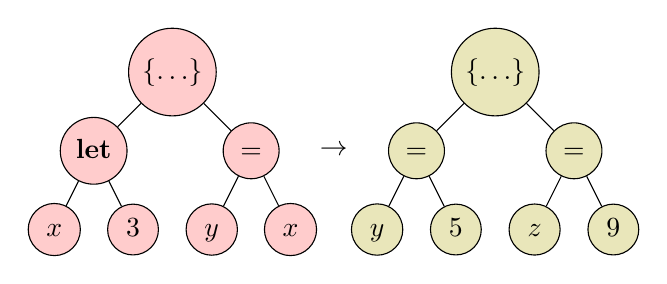
\begin{tikzpicture}
    \node[varnode, colorDel] (del_block) {$\{\ldots\}$};
    \node[varnode, colorDel] (del_stmt1) at ($(del_block)+(-1,-1)$)
{$\textbf{let}$};
    \node[varnode, colorDel] (del_stmt2) at ($(del_block)+(1,-1)$) {$=$};
    \node[varnode, colorDel] (del_x) at ($(del_stmt1)+(-0.5,-1)$) {$x$};
    \node[varnode, colorDel] (del_three) at ($(del_stmt1)+(0.5,-1)$) {$3$};
    \node[varnode, colorDel] (del_y) at ($(del_stmt2)+(-0.5,-1)$) {$y$};
    \node[varnode, colorDel] (del_yx) at ($(del_stmt2)+(0.5,-1)$) {$x$};
    \draw (del_block) -- (del_stmt1);
    \draw (del_block) -- (del_stmt2);
    \draw (del_stmt1) -- (del_x);
    \draw (del_stmt1) -- (del_three);
    \draw (del_stmt2) -- (del_y);
    \draw (del_stmt2) -- (del_yx);

    \node[varnode, colorIns] (ins_block) at ($(del_block)+(4.1,0)$)
{$\{\ldots\}$};
    \node[varnode, colorIns] (ins_stmt1) at ($(ins_block)+(-1,-1)$) {$=$};
    \node[varnode, colorIns] (ins_stmt2) at ($(ins_block)+(1,-1)$) {$=$};
    \node[varnode, colorIns] (ins_y) at ($(ins_stmt1)+(-0.5,-1)$) {$y$};
    \node[varnode, colorIns] (ins_five) at ($(ins_stmt1)+(0.5,-1)$) {$5$};
    \node[varnode, colorIns] (ins_z) at ($(ins_stmt2)+(-0.5,-1)$) {$z$};
    \node[varnode, colorIns] (ins_nine) at ($(ins_stmt2)+(0.5,-1)$) {$9$};
    \draw (ins_block) -- (ins_stmt1);
    \draw (ins_block) -- (ins_stmt2);
    \draw (ins_stmt1) -- (ins_y);
    \draw (ins_stmt1) -- (ins_five);
    \draw (ins_stmt2) -- (ins_z);
    \draw (ins_stmt2) -- (ins_nine);

    \node (arrow) at ($(del_stmt2)!0.5!(ins_stmt1)$) {$\rightarrow$};
\end{tikzpicture}
\end{minipage}\hfill
\begin{minipage}{0.45\textwidth}
\centering\begin{tikzpicture}
    \node[varnode] (spine_block) {$\{\ldots\}$};
    \node[changenode, colorDel] (spine_stmt1) at ($(spine_block)+(-2.5,-1.6)$)
{\tikz{
        \node[varnode] (del_stmt) {$\textbf{let}$};
        \node[varnode] (del_x) at ($(del_stmt)+(-0.5,-1)$) {$x$};
        \node[varnode] (del_three) at ($(del_stmt)+(0.5,-1)$) {$3$};
        \draw (del_stmt) -- (del_x);
        \draw (del_stmt) -- (del_three);
    }};
    \node[varnode] (spine_stmt2) at ($(spine_block)+(-0.25,-1.1)$) {$=$};
    \node[changenode, colorIns] (spine_stmt3) at ($(spine_block)+(2.5,-1.6)$)
{\tikz{
        \node[varnode] (ins_stmt) at ($(ins_block)+(1,-1)$) {$=$};
        \node[varnode] (ins_z) at ($(ins_stmt)+(-0.5,-1)$) {$z$};
        \node[varnode] (ins_nine) at ($(ins_stmt)+(0.5,-1)$) {$9$};
        \draw (ins_stmt) -- (ins_z);
        \draw (ins_stmt) -- (ins_nine);
    }};{};
    \node[varnode] (spine_y) at ($(spine_stmt2)+(-0.75,-1)$) {$y$};
    \node[changenode] (change_y) at ($(spine_stmt2)+(0.75,-1)$) {\tikz{
        \node[varnode, colorDel] (x) {$x$};
        \node[varnode, colorIns] (five) at ($(x)+(1.2,0)$) {$5$};
        \node (arrow) at ($(x)!0.5!(five)$) {$\rightarrow$};
    }};
    \draw (spine_block) -- (spine_stmt1);
    \draw (spine_block) -- (spine_stmt2);
    \draw (spine_block) -- (spine_stmt3);
    \draw (spine_stmt2) -- (spine_y);
    \draw (spine_stmt2) -- (change_y);
\end{tikzpicture}
\end{minipage}
\caption{The change $\change{\{ \keyword{let}\ x=3; y=x\}}{\{ y=5; z=9 \}}$
becomes $\{\del{\keyword{let}\ x=3;}\ y = \change{x}{5}; \ins{z = 9}\}$
after spine merging and sequence alignment.}
\label{fig:spine_seq_align}
\end{figure}

Computing the spine alignment is the expansive part of our algorithm because it
is quadratic $O(nm)$ if $n$ is the number of nodes in the insertion tree and
$m$ in the deletion tree.

Moreover, the choice of the heuristic cost function is somehow arbitrary,
although the simple cost model where each leaf deleted or inserted cost 2 and
each leaf in the final spine cost 1 seem reasonable and produce satisfying
results.

\paragraph{Elisions}
Our difference algorithm could stop here as it already produces a reasonable
difference tree. However, it would fail to detect moved code, and thus, it
would not significantly improve the representation of refactorings.
Therefore, we add an elision computation step after the spine alignment that
tries to catch moved parts of a source tree.

An elision can be seen as code moved from a location in $d$ into another
location in $i$, but with the actual content temporarily forgotten inside what
we call a meta-variable. In this paper, we will denote these meta-variables by
Greek letters.

\begin{figure}[ht]
\begin{minipage}{0.49\textwidth}
\centering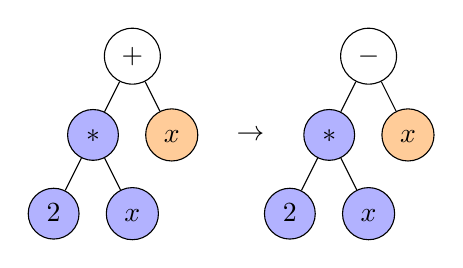
\begin{tikzpicture}
    \node[varnode] (del_plus) {$+$};
    \node[varnode, colorA] (del_times) at ($(del_plus)+(-0.5,-1)$) {$*$};
    \node[varnode, colorB] (del_one) at ($(del_plus)+(0.5,-1)$) {$x$};
    \node[varnode, colorA] (del_two) at ($(del_times)+(-0.5,-1)$) {$2$};
    \node[varnode, colorA] (del_three) at ($(del_times)+(0.5,-1)$) {$x$};
    \draw (del_plus) -- (del_times);
    \draw (del_plus) -- (del_one);
    \draw (del_times) -- (del_two);
    \draw (del_times) -- (del_three);

    \node[varnode] (ins_minus) at ($(del_plus)+(3,0)$) {$-$};
    \node[varnode, colorA] (ins_times) at ($(ins_minus)+(-0.5,-1)$) {$*$};
    \node[varnode, colorB] (ins_one) at ($(ins_minus)+(0.5,-1)$) {$x$};
    \node[varnode, colorA] (ins_two) at ($(ins_times)+(-0.5,-1)$) {$2$};
    \node[varnode, colorA] (ins_three) at ($(ins_times)+(0.5,-1)$) {$x$};
    \draw (ins_minus) -- (ins_times);
    \draw (ins_minus) -- (ins_one);
    \draw (ins_times) -- (ins_two);
    \draw (ins_times) -- (ins_three);

    \node (arrow) at ($(del_one)!0.5!(ins_times)$) {$\rightarrow$};
\end{tikzpicture}
\end{minipage}\hfill
\begin{minipage}{0.49\textwidth}
\centering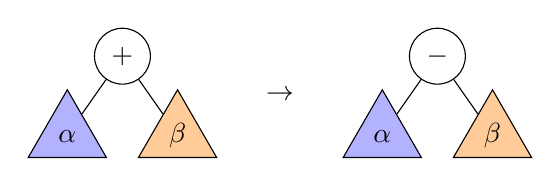
\begin{tikzpicture}
    \node[varnode] (del_plus) {$+$};
    \node[mvnode, colorA] (del_alpha) at ($(del_plus)+(-0.7,-1)$) {$\alpha$};
    \node[mvnode, colorB] (del_beta) at ($(del_plus)+(0.7,-1)$) {$\beta$};
    \draw (del_plus) -- (del_alpha);
    \draw (del_plus) -- (del_beta);

    \node[varnode] (ins_minus) at ($(del_plus)+(4,0)$) {$-$};
    \node[mvnode, colorA] (ins_alpha) at ($(ins_minus)+(-0.7,-1)$) {$\alpha$};
    \node[mvnode, colorB] (ins_beta) at ($(ins_minus)+(0.7,-1)$) {$\beta$};
    \draw (ins_minus) -- (ins_alpha);
    \draw (ins_minus) -- (ins_beta);

    \node (arrow) at
($($(del_beta)!0.5!(del_plus)$)!0.5!($(ins_alpha)!0.5!(ins_minus)$)$)
{$\rightarrow$};
\end{tikzpicture}
\end{minipage}
\caption{The change $\change{(2*x)+x}{(2*x)-x}$ becomes $\change{\alpha+\beta}
{\alpha-\beta}$ after meta-variable elision.}
\label{fig:metavar_elision}
\end{figure}

Figure~\ref{fig:metavar_elision} illustrate such an elision for a change where
the programmer transformed a $+$ into a $-$. The subexpression $(2*x)$ is
elided as $\alpha$ and the subexpression $x$ is elided as $\beta$, therefore
the result only talks about the operator modification, and is a more generic
change.

A given meta-variable can occur more that twice (at least once in deletion and
once in insertion but maybe more). Therefore, code displacements have multiple
sources and multiple targets, but a given meta-variable will always represent
an
identical code sub-tree. The fact that a given meta-variable can have multiple
sources may seem unsatisfying, but it makes it possible to detect code
displacements automatically without arbitrary choices. Moreover, thanks to
that,
we can easily revert a difference by simply exchanging the deleted and inserted
trees.

As an example, the change $\change{x*y}{x+x}$ will be elided as
$\change{\alpha*y}{\alpha+\alpha}$ because $x$ was duplicated.
Conversely, the reverse change $\change{x+x}{x*y}$ will become
$\change{\alpha+\alpha}{\alpha*y}$ as it is hard to tell automatically from
which $x$ the kept one comes from.

This code displacement notion is especially important for capturing refactoring
in differences to merge them correctly with other commits later.

In order to compute it we reuse the hashes computed earlier, and ensure that
each spine node keeps both the hash for its deleted and inserted part.
We then take the intersection of hashes ocurring at least once in deletion and
once in insertion. This forms the possible elisions set. However since
performing an elision will remove all the underlying nodes, we cannot
necessarily elide all the nodes in the set.

There we again took an arbitrary choice to favor elisions occurring near the
root first. So, from the root, we check if each node has an hash in the
possible elision set, and add it to a wanted elision set if it is the case, or
recurse in its children if not. Then we take the intersection of the wanted
elision set for insertion and for deletion and use it as the actual elision set.

Then when we know which elisions need to be performed we can traverse the tree
one last time to replace the nodes by metavariables. If an elision (on
deletion or insertion hash) should occur on a spine node, we have to split it
into a deletion tree and an insertion tree before performing the elision. This
is always possible and rather easy to do if we keep the required information on
unchanged nodes.


\paragraph{Intuitive semantics of difference tree}
\label{sec:diff_application}

We can see a syntactic difference tree as a partial function turning a syntax
tree into another syntax tree. A valid difference between $d$ and $i$ is
therefore a function that is at least mapping $d$ to $i$, but it is
also defined on some other trees sharing some relevant structure with $d$.

In order to apply a difference tree to a syntax tree, we can use a simple
algorithm:
\begin{itemize}
 \item First check that the syntax tree corresponds to the difference spine and
deleted nodes. Each constuctor must be identical, except for unchanged nodes
and meta-variables, that can allow any subtree to replace them. Remember how
these holes where filled for later processing.
 \item Check that identical metavariables are consistently replaced by
identical trees, and derive a map function from meta-variables to subtrees.
 \item Return the spine and inserted part of the difference tree, replacing
meta-variables and unchanged nodes with their previously computed subtrees.
\end{itemize}

We call domain of a difference tree the set of syntax tree on which it can be
applied.

\begin{figure}[ht]
\begin{minipage}{0.42\textwidth}
\centering\begin{tikzpicture}
    \node[varnode] (spine_block) {$\{\ldots\}$};
    \node[changenode, colorDel] (spine_stmt1) at ($(spine_block)+(-2.5,-1.6)$)
{\tikz{
        \node[varnode] (del_stmt) {$\textbf{let}$};
        \node[varnode] (del_x) at ($(del_stmt)+(-0.5,-1)$) {$x$};
        \node[mvnode, blue] (del_three) at ($(del_stmt)+(0.5,-1)$)
{\color{black}$\alpha$};
        \draw (del_stmt) -- (del_x);
        \draw (del_stmt) -- (del_three);
    }};
    \node[varnode] (spine_stmt2) at ($(spine_block)+(-0.25,-1.1)$) {$=$};
    \node[changenode, colorIns] (spine_stmt3) at ($(spine_block)+(2.5,-1.6)$)
{\tikz{
        \node[varnode] (ins_stmt) at ($(ins_block)+(1,-1)$) {$=$};
        \node[varnode] (ins_z) at ($(ins_stmt)+(-0.5,-1)$) {$z$};
        \node[varnode] (ins_nine) at ($(ins_stmt)+(0.5,-1)$) {$9$};
        \draw (ins_stmt) -- (ins_z);
        \draw (ins_stmt) -- (ins_nine);
    }};{};
    \node[mvnode, inner sep=1] (spine_y) at ($(spine_stmt2)+(-0.75,-1)$)
{$\id$};
    \node[changenode] (change_y) at ($(spine_stmt2)+(0.75,-1)$) {\tikz{
        \node[varnode, colorDel] (x) {$x$};
        \node[mvnode, blue, colorIns] (five) at ($(x)+(1.2,0)$)
{\color{black}$\alpha$};
        \node (arrow) at ($(x)!0.5!(five)$) {$\rightarrow$};
    }};
    \draw (spine_block) -- (spine_stmt1);
    \draw (spine_block) -- (spine_stmt2);
    \draw (spine_block) -- (spine_stmt3);
    \draw (spine_stmt2) -- (spine_y);
    \draw (spine_stmt2) -- (change_y);
\end{tikzpicture}
\end{minipage}
$\left(
\begin{minipage}{0.25\textwidth}
\centering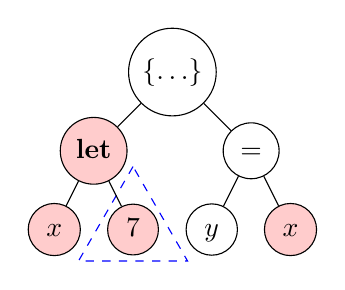
\begin{tikzpicture}
    \node[varnode] (spine_block) {$\{\ldots\}$};
    \node[varnode, colorDel] (del_stmt) at ($(spine_block)+(-1,-1)$)
{$\textbf{let}$};
    \node[varnode, colorDel] (del_x) at ($(del_stmt)+(-0.5,-1)$) {$x$};
    \node[varnode, colorDel] (del_three) at ($(del_stmt)+(0.5,-1)$) {$7$};
    \node[mvnode, dashed, minimum size=1.6cm, color=blue] (del_mv) at
($(del_stmt)+(0.5,-1)$) {};
    \draw (del_stmt) -- (del_x);
    \draw (del_stmt) -- (del_three);
    \node[varnode] (spine_stmt2) at ($(spine_block)+(1,-1)$) {$=$};
    \node[varnode] (spine_y) at ($(spine_stmt2)+(-0.5,-1)$) {$y$};
    \node[varnode, colorDel] (change_y) at ($(spine_stmt2)+(0.5,-1)$) {$x$};
    \draw (spine_block) -- (del_stmt);
    \draw (spine_block) -- (spine_stmt2);
    \draw (spine_stmt2) -- (spine_y);
    \draw (spine_stmt2) -- (change_y);
\end{tikzpicture}
\end{minipage}\right)$=
\begin{minipage}{0.25\textwidth}
\centering\begin{tikzpicture}
    \node[varnode] (spine_block) {$\{\ldots\}$};
    \node[varnode] (spine_stmt2) at ($(spine_block)+(-1,-1)$) {$=$};
    \node[varnode, colorIns] (ins_stmt) at ($(spine_block)+(1,-1)$) {$=$};
    \node[varnode, colorIns] (ins_z) at ($(ins_stmt)+(-0.5,-1)$) {$z$};
    \node[varnode, colorIns] (ins_nine) at ($(ins_stmt)+(0.5,-1)$) {$9$};
    \draw (ins_stmt) -- (ins_z);
    \draw (ins_stmt) -- (ins_nine);
    \node[varnode] (spine_y) at ($(spine_stmt2)+(-0.5,-1)$) {$y$};
    \node[varnode, colorIns] (change_y) at ($(spine_stmt2)+(0.5,-1)$) {$7$};
    \node[mvnode, minimum size=1.6cm, color=blue] (del_mv) at
($(del_stmt)+(0.5,-1)$) {};
    \draw (spine_block) -- (spine_stmt2);
    \draw (spine_block) -- (ins_stmt);
    \draw (spine_stmt2) -- (spine_y);
    \draw (spine_stmt2) -- (change_y);
\end{tikzpicture}
\end{minipage}
\caption{The syntactic difference $\{\del{\keyword{let}\ x=\alpha;}\ \id =
\change{x}{\alpha}; \ins{z = 9}\}$ applied to $\{\keyword{let}\ x=7;\ y =
x\}$ gives $\{y = 7;\ z = 9\}$.}
\label{fig:apply_diff}
\end{figure}

On Figure~\ref{fig:apply_diff}, we can see that the tree applied to the
difference correctly share relevant structure and the subtree $7$ matches the
meta-variable $\alpha$. Therefore the result is shows a $7$ where the
metavariable is inserted.

However, $3 + 4$ is not in the domain of neither $\change{3 - \alpha}{9 +
\alpha}$ (non-matching constructions) nor $\change{\alpha + \alpha}{\alpha -
\alpha}$ ($3$ and $4$ are different subtrees and cannot be both placed in the
same meta-variable).

\paragraph{Formal semantics of difference trees}

The implied function of a difference tree is formally defined as follows: let
us suppose that we have $\Gamma$ a function from meta-variables (occurring in
the difference tree) to syntax trees. In practice, $\Gamma$ is constrained
enough to be always uniquely inferred by the algorithm presented in the
previous paragraph because each meta-variable occur at least once.

We denote by $h :: \vec{t}$ a sequence containing at least one element, and by
$[]$ the empty sequence.

A judgment $\Gamma \vdash t(d) = i$ means that under meta-variable replacements
$\Gamma$, the difference tree $t$ applied to $d$ is well defined and returns
$i$. The judgment $\Gamma \vdash c(d)$ means that the change $c$ is compatible
with the original tree $d$ under meta-variable replacements $\Gamma$.

We extend $\Gamma$ on $\typ{ChangeTree}$, as the function that recursively
replaces any meta-variable in a $\typ{ChangeTree}$ by the corresponding
replacement syntax tree thus producing a $\typ{SyntaxTree}$.

Then, we have the following syntax-driven rules:

\begin{minipage}{0.45\textwidth}

\begin{prooftree}
 \AxiomC{}
 \RightLabel{\textsc{Id}}
 \UnaryInfC{$\Gamma \vdash \id(t) = t$}
\end{prooftree}

\begin{prooftree}
 \AxiomC{$\Gamma \vdash \vec{t}(\vec{d_t}) = \vec{i_t}$}
 \RightLabel{\textsc{Spine}}
 \UnaryInfC{$\Gamma \vdash \synnode{n}{\vec{t}}(\synnode{n}{\vec{d_t}}) =
\synnode{n}{\vec{i_t}}$}
\end{prooftree}


\begin{prooftree}
 \AxiomC{$\Gamma \vdash t(d) = i$}
 \AxiomC{$\Gamma \vdash \vec{r}(\vec{d_r}) = \vec{i_r}$}
 \RightLabel{\textsc{SeqZip}}
 \BinaryInfC{$\Gamma \vdash
(\synfield{f}{t}::\vec{r})(\synfield{f}{d}::\vec{d_r}) =
\synfield{f}{i}::\vec{i_r}$}
\end{prooftree}

\begin{prooftree}
 \AxiomC{$\Gamma \vdash \vec{r}(\vec{d_r}) = \vec{i_r}$}
 \RightLabel{\textsc{SeqIns}}
 \UnaryInfC{$\Gamma \vdash (\ins{\synfield{f}{c}}::\vec{r})(\vec{d_r}) =
\synfield{f}{\Gamma(c)} :: \vec{i_r}$}
\end{prooftree}

\begin{prooftree}
 \AxiomC{$\Gamma \vdash \vec{c_t}(\vec{d_t})$}
 \RightLabel{\textsc{DelSyn}}
 \UnaryInfC{$\Gamma \vdash \synnode{n}{\vec{c_t}}
(\synnode{n}{\vec{d_t}})$}
\end{prooftree}

\begin{prooftree}
 \AxiomC{}
 \RightLabel{\textsc{DelEmpty}}
 \UnaryInfC{$\Gamma \vdash []([])$}
\end{prooftree}

\end{minipage}\hfill\begin{minipage}{0.45\textwidth}

\begin{prooftree}
 \AxiomC{$\Gamma \vdash d(t)$}
 \RightLabel{\textsc{Change}}
 \UnaryInfC{$\Gamma \vdash (\change{d}{i})(t) = \Gamma(i)$}
\end{prooftree}

\begin{prooftree}
 \AxiomC{}
 \RightLabel{\textsc{SameLeaf}}
 \UnaryInfC{$\Gamma \vdash \syntoken{l}(\syntoken{l}) = \syntoken{l}$}
\end{prooftree}

\begin{prooftree}
 \AxiomC{$\Gamma \vdash c(d)$}
 \AxiomC{$\Gamma \vdash \vec{r}(\vec{d_r}) = \vec{i_r}$}
 \RightLabel{\textsc{SeqDel}}
 \BinaryInfC{$\Gamma \vdash
(\del{\synfield{f}{c}}::\vec{r})(\synfield{f}{d}::\vec{d_r}) = \vec{i_r}$}
\end{prooftree}

\begin{prooftree}
 \AxiomC{}
 \RightLabel{\textsc{SeqEmpty}}
 \UnaryInfC{$\Gamma \vdash []([]) = []$}
\end{prooftree}

\begin{prooftree}
 \AxiomC{$\Gamma(\alpha) = d$}
 \RightLabel{\textsc{DelMv}}
 \UnaryInfC{$\Gamma \vdash \alpha(d)$}
\end{prooftree}

\begin{prooftree}
 \AxiomC{}
 \RightLabel{\textsc{DelLeaf}}
 \UnaryInfC{$\Gamma \vdash \syntoken{l}(\syntoken{l})$}
\end{prooftree}

\begin{prooftree}
 \AxiomC{$\Gamma \vdash c(d)$}
 \AxiomC{$\Gamma \vdash \vec{r}(\vec{d_r})$}
 \RightLabel{\textsc{DelZip}}
 \BinaryInfC{$\Gamma \vdash
(\synfield{f}{c}::\vec{r})(\synfield{f}{d}::\vec{d_r})$}
\end{prooftree}
\end{minipage}

\vspace{1em}
Syntax trees for which no well-founded judgment exist are outside the domain of
the difference tree.

\section{Merging syntactic difference trees}
A merging algorithm takes two differences and produce another difference that
contains all the changes from inputs if they are compatible or show where they
are incompatible otherwise. This high-level description is underspecified
because semantically combining changes only has an intuitive meaning depending
on the implicit idea of what each commit does (often summarized in English in
the commit message). Therefore, these algorithms are necessarily somehow
arbitrary because they force a particular meaning for change combination. This
does not mean that they are all equivalent, their definition for combination is
more or less aligned with usual real-life commits.

In this paper, our arbitrary choice is to focus on syntax to align differences
(because we think that it often follows the intuition of the developers) and let
changes follow moved code (because it allow seamless merging of a large class of
refactoring operations). These two principles will be explained further in
Section~\ref{sec:merge_principles}. That said, we avoid further arbitrary
choices that could favor one of the input tree over the other.

We will denote $t_1 \merge t_2$ the result of our merge algorithm on difference
trees $t_1$ and $t_2$.

Often the two input differences will not share the same domain. The output can
therefore only be defined on the intersection of these domains. It makes no
sense to merge differences whose domain are disjoint. In a standard setup, both
input differences were computed on a common base and therefore we are sure that
the merge output is at least defined for this base program.

On top of that, the merging operation can and will regularly produce conflicts
whenever someone wants to merge syntactically incompatible changes.
Therefore we need to extend our grammar of differences to include these
conflicts. Insertions and deletions do not trigger the same kind of conflicts,
so we have to break the symmetry between them. It leads to the following
grammar:
\begin{typgrammar}
  \typ{MergedSpineTree} &::= \typarg{Tree}{\typ{MergedSpineChild}} \typsep
    \id \typsep
    \change{\typ{DelTree}}{\typ{ChangeTree}}\\
  \typ{MergedSpineChild} &::= \typarg{Subtree}{\typ{MergedSpineTree}} \typsep
    \del{\typarg{Subtree}{\typ{DelTree}}} \typsep
    \DelConflict(field, \typ{DelTree}, \typ{ChangeTree})\\
    &\typsep \ins{\typarg{Subtree}{\typ{ChangeTree}}} \typsep
    \OrdConflict(\vec{\typarg{Subtree}{\typ{ChangeTree}}},
        \vec{\typarg{Subtree}{\typ{ChangeTree}}})\\
   \typ{DelTree} &::= \typarg{Tree}{\typarg{Subtree}{\typ{DelTree}}} \typsep
    \alpha \typsep
    \MvConflict(\alpha, \typ{DelTree}, \typ{ChangeTree})\\
\end{typgrammar}

Conflict represent parts that couldn't be merged and therefore prevent
application of the difference on any tree. They can come from four different
sources:
\begin{itemize}
  \item Insertion conflict ($\InsConflict$) simply represent two different
insertions that were about to be merged in the same place.
  \item Deletion conflict ($\DelConflict$) appears where one commit deletes a
node while the other one had changes in it.
  \item Insert order conflict ($\OrdConflict$) is caused by two insertions
taking place at the same location. As the merge operation is never performing
any choice, it cannot arbitrarily order them. Moreover, a possible resolution
can also be to keep only one of the two inserted elements.
  \item Meta-variable conflict ($\MvConflict$) is triggered when a meta-variable
appears more than once in deletion tree, and the inlined insertions in each
occurrences differ, therefore not giving a consistent replacement. This will be
explained in further details later.
\end{itemize}

As this syntax is an extension, the syntax differences presented earlier can be
directly reinterpreted in this grammar and conversely, differences without
conflicts still follow the old grammar.

\subsection{Design principles for our merging algorithm}
\label{sec:merge_principles}
\paragraph{Align changes following the syntax}
As the domains of both input differences must overlap, we always can align their
spine and deletion trees. This therefore also give a full change alignment as
insertions are attached on a specific place in the spine (however it sometimes
creates conflicts). By doing so, we respect the property that no commit is
favored because alignment comes from shared nodes.

The first step of the merging algorithm aligns the common spine nodes and unwind
the remaining ones that are facing a change. On
Figure~\ref{fig:spine_alignment}, we can see that only the nodes $x$ and $+$ are
in both spines. Therefore, spine nodes $y$ and $*$ in the orange tree must be
unwinded producing white nodes as a change before merging.

\begin{figure}[ht]
\begin{minipage}{0.33\textwidth}
\centering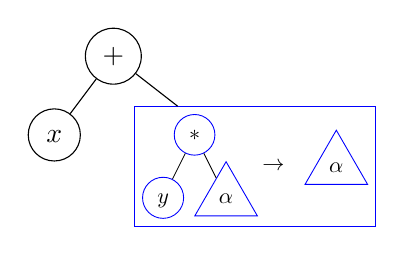
\begin{tikzpicture}
\node[varnode] (plus) {$+$};
\node[varnode] (x) at ($(plus)+(-0.75,-1)$) {$x$};
\node[changenode, color=blue] (change) at ($(plus)+(1.8,-1.4)$)
{\tikz[color=black]{
    \node[varnode, color=blue] (del_times) {$\color{black}*$};
    \node[varnode, color=blue] (del_y) at ($(del_times)+(-0.5,-1)$)
{$\color{black}y$};
    \node[mvnode, color=blue] (del_alpha) at ($(del_times)+(0.5,-1)$)
{$\color{black}\alpha$};
    \draw (del_times) -- (del_y);
    \draw (del_times) -- (del_alpha);

    \node[mvnode, color=blue] (ins_alpha) at ($(del_times)!0.5!(del_alpha)+(2,
0)$) {$\color{black}\alpha$};
    \node (arrow) at ($(del_times)!0.5!(del_alpha)!0.5!(ins_alpha)$)
{$\rightarrow$};
}};
\draw (plus) -- (x);
\draw (plus) -- (change);
\end{tikzpicture}
\end{minipage}\hfill
\begin{minipage}{0.33\textwidth}
\centering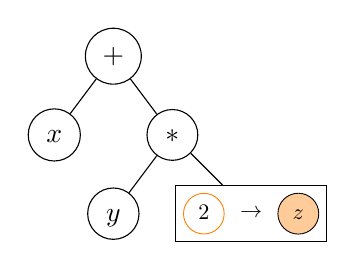
\begin{tikzpicture}
\node[varnode] (plus) {$+$};
\node[varnode] (x) at ($(plus)+(-0.75,-1)$) {$x$};
\node[varnode] (times) at ($(plus)+(0.75,-1)$) {$*$};
\node[varnode] (y) at ($(times)+(-0.75,-1)$) {$y$};
\node[changenode] (change) at ($(times)+(1,-1)$) {\tikz{
    \node[varnode, color=orange] (two) {$\color{black}2$};
    \node[varnode, colorB] (z) at ($(two)+(1.5, 0)$) {$z$};
    \node (arrow) at ($(two)!0.5!(z)$) {$\rightarrow$};
}};
\draw (plus) -- (x);
\draw (plus) -- (times);
\draw (times) -- (y);
\draw (times) -- (change);
\end{tikzpicture}
\end{minipage}
\hfill
\begin{minipage}{0.33\textwidth}
\centering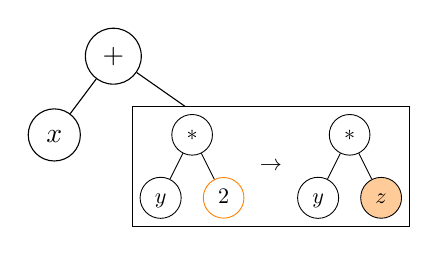
\begin{tikzpicture}
\node[varnode] (plus) {$+$};
\node[varnode] (x) at ($(plus)+(-0.75,-1)$) {$x$};
\node[changenode] (change) at ($(plus)+(2,-1.4)$) {\tikz{
    \node[varnode] (del_times) {$\color{black}*$};
    \node[varnode] (del_y) at ($(del_times)+(-0.5,-1)$) {$\color{black}y$};
    \node[varnode, color=orange] (del_two) at ($(del_times)+(0.5,-1)$)
{$\color{black}2$};
    \draw (del_times) -- (del_y);
    \draw (del_times) -- (del_two);

    \node[varnode] (ins_times) at ($(del_times)+(2.5, 0)$) {$*$};
    \node[varnode] (ins_y) at ($(ins_times)+(-0.5,-1)$) {$y$};
    \node[varnode, colorB] (ins_z) at ($(ins_times)+(0.5,-1)$) {$z$};
    \draw (ins_times) -- (ins_y);
    \draw (ins_times) -- (ins_z);

    \node (arrow) at
($($(del_times)!0.5!(del_two)$)!0.5!($(ins_times)!0.5!(ins_y)$)$)
{$\rightarrow$};
}};
\draw (plus) -- (x);
\draw (plus) -- (change);
\end{tikzpicture}
\end{minipage}
\caption{Spine alignment: We unwind the spine of the second tree producing the
third in order to be aligned with first.}
\label{fig:spine_alignment}
\end{figure}

If a difference sub-tree is aligned with an unchanged node ($\square$), we keep
the changed one only. This is quite an intuitive notion of combination with
unchanged node yielding to the important property $t \merge \square = t$.

If however we need to unwind the spine with an unchanged node, we will generate
a fresh meta-variable $\alpha$ and replace $\id$ by $\change{\alpha}{\alpha}$.

When merging deletion trees, either both inputs agree on a common syntax node,
or one of them has a meta-variable. In the latter case, we have to produce the
most specific deletion tree, therefore keeping the non meta-variable sub-tree.
This is the consensus between the two differences as the one with meta-variable
accepts any sub-tree at this point while the other accepts only the kept one. We
must remember that the meta-variable has been deleted for a more specific tree
and replace its remaining occurrences in deletions (always) and insertions
(except in case of the inlining explained later).

%I probably should add an example here, but it is hard to find one that is
%non-conflicting, not complex and without inlining

When merging insertion trees, however, meta-variables always conflict with each
other because they correspond to specific subtrees instead of capturing one.
Therefore, we only merge fully identical nodes.

\paragraph{Inlining changes inside meta-variables}
When dealing with meta-variables, that represent a multi-source
multi-target code move, our merging algorithm will try to push changes
toward the destination of the code movement.

This is done in a two-phase way. First, if we have two changes facing each other
we try to inline one of them inside the deletion tree of the other, by allowing
differences wherever we have a meta-variable. By doing so, we check if the
changes of one difference are fully contained inside code that will be moved by
the other.

Then, we check that these inlined changes are consistent across different
occurrences of the same meta-variable. If they are, we replace all occurrences
of the meta-variable by the obtained insertion. If they are not, we generate a
$\MvConflict$ conflict on each deleted $\alpha$ with the corresponding facing
insertion.

\begin{figure}[ht]
\begin{minipage}{0.49\textwidth}
\centering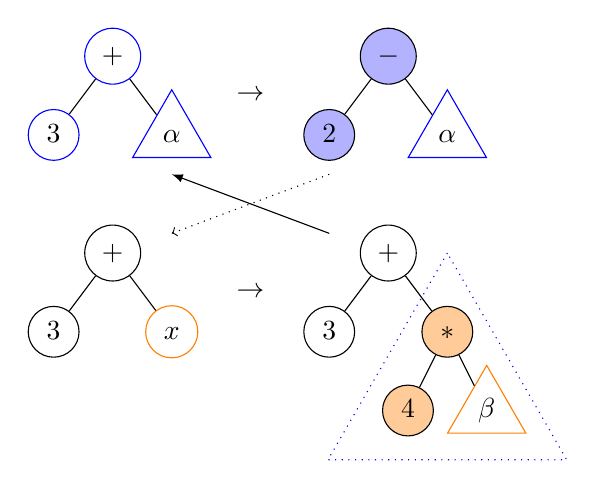
\begin{tikzpicture}
    \node[varnode, color=blue] (adel_plus) {$\color{black}+$};
    \node[varnode, color=blue] (adel_three) at ($(adel_plus)+(-0.75,-1)$)
{$\color{black}3$};
    \node[mvnode, color=blue] (adel_alpha) at ($(adel_plus)+(0.75,-1)$)
{$\color{black}\alpha$};
    \draw (adel_plus) -- (adel_three);
    \draw (adel_plus) -- (adel_alpha);

    \node[varnode, colorA] (ains_minus) at ($(adel_plus)+(3.5,0)$) {$-$};
    \node[varnode, colorA] (ains_two) at ($(ains_minus)+(-0.75,-1)$) {$2$};
    \node[mvnode, color=blue] (ains_alpha) at ($(ains_minus)+(0.75,-1)$)
{$\color{black}\alpha$};
    \draw (ains_minus) -- (ains_two);
    \draw (ains_minus) -- (ains_alpha);

    \node (aarrow) at
($($(adel_alpha)!0.5!(adel_plus)$)!0.5!($(ains_two)!0.5!(ains_minus)$)$)
{$\rightarrow$};

    \node[varnode] (bdel_plus) at ($(adel_plus)+(0,-2.5)$) {$+$};
    \node[varnode] (bdel_three) at ($(bdel_plus)+(-0.75,-1)$) {$3$};
    \node[varnode, color=orange] (bdel_x) at ($(bdel_plus)+(0.75,-1)$)
{$\color{black}x$};
    \draw (bdel_plus) -- (bdel_three);
    \draw (bdel_plus) -- (bdel_x);

    \node[varnode] (bins_plus) at ($(bdel_plus)+(3.5,0)$) {$+$};
    \node[varnode] (bins_three) at ($(bins_plus)+(-0.75,-1)$) {$3$};
    \node[varnode, colorB] (bins_times) at ($(bins_plus)+(0.75,-1)$) {$*$};
    \node[varnode, colorB] (bins_four) at ($(bins_times)+(-0.5,-1)$) {$4$};
    \node[mvnode, color=orange] (bins_beta) at ($(bins_times)+(0.5,-1)$)
{$\color{black}\beta$};
    \node[mvnode, dotted, minimum size=3.5cm, color=blue] (bins_alpha) at
($(bins_times)+(0,-0.75)$) {};
    \draw (bins_plus) -- (bins_three);
    \draw (bins_plus) -- (bins_times);
    \draw (bins_times) -- (bins_four);
    \draw (bins_times) -- (bins_beta);

    \node (barrow) at
($($(bdel_x)!0.5!(bdel_plus)$)!0.5!($(bins_three)!0.5!(bins_plus)$)$)
{$\rightarrow$};

    \draw[>=latex,->] ($(bins_plus)+(-0.75, 0.25)$) -- ($(adel_alpha)+(0,
-0.5)$);
    \draw[->,dotted] ($(ains_two)+(0, -0.5)$) -- ($(bdel_plus)+(0.75, 0.25)$);
\end{tikzpicture}
\end{minipage}\hfill
\begin{minipage}{0.49\textwidth}
\centering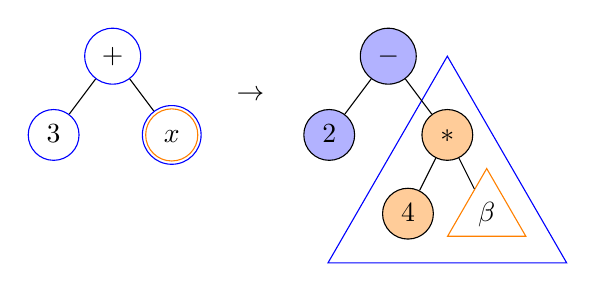
\begin{tikzpicture}
    \node[varnode, color=blue] (del_plus) {$\color{black}+$};
    \node[varnode, color=blue] (del_three) at ($(del_plus)+(-0.75,-1)$)
{$\color{black}3$};
    \node[varnode, color=orange] (del_x) at ($(del_plus)+(0.75,-1)$)
{$\color{black}x$};
    \node[varnode, color=blue] (del_x_out) at (del_x) {\phantom{M}};
    \draw (del_plus) -- (del_three);
    \draw (del_plus) -- (del_x_out);

    \node[varnode, colorA] (ins_minus) at ($(del_plus)+(3.5,0)$) {$-$};
    \node[varnode, colorA] (ins_two) at ($(ins_minus)+(-0.75,-1)$) {$2$};
    \node[varnode, colorB] (ins_times) at ($(ins_minus)+(0.75,-1)$) {$*$};
    \node[varnode, colorB] (ins_four) at ($(ins_times)+(-0.5,-1)$) {$4$};
    \node[mvnode, color=orange] (ins_beta) at ($(ins_times)+(0.5,-1)$)
{$\color{black}\beta$};
    \node[mvnode, minimum size=3.5cm, color=blue] (ins_alpha) at
($(ins_times)+(0,-0.75)$) {};
    \draw (ins_minus) -- (ins_two);
    \draw (ins_minus) -- (ins_times);
    \draw (ins_times) -- (ins_four);
    \draw (ins_times) -- (ins_beta);

    \node (arrow) at
($($(del_x)!0.5!(del_plus)$)!0.5!($(ins_two)!0.5!(ins_minus)$)$)
{$\rightarrow$};
\end{tikzpicture}
\end{minipage}
\caption{Example of successful meta-variable inlining}
\label{fig:metavar_inlining}
\end{figure}

On Figure~\ref{fig:metavar_inlining}, we can see that the orange change can be
inlined in the blue deletion tree. Indeed, if we compare their tree, all
differences occur under meta-variable $\alpha$. Conversely, the blue change
cannot be inlined because the inserted node $-$ in blue cannot be merged with
deleted node $+$ in the orange tree. If there are no other occurrences of
$\alpha$, or the corresponding inlined tree is always $4*\beta$, we can replace
every $\alpha$ by $4*\beta$, producing the tree on the right.

To avoid making any arbitrary choice, meta-variable inlining is ignored if both
changes could be inlined in the other. This brings back the important property
that merging a change with itself does not change anything (think of
$\change{\alpha}{f(\alpha)}$ merged with itself).

\subsubsection{Algorithm for merging differences}
\label{sec:syntactic_merge_algo}

Following the principles exposed above, our algorithm follows these steps:
\begin{enumerate}
 \item Ensure that all the meta-variables used in both programs are
   disjoint by alpha-renaming whenever necessary. This prevent merging different
similarly named meta-variables that correspond to different subtrees.

 \item Align the spines of both difference trees as explained in
Section~\ref{sec:merge_principles}. This step also aligns the sequences in the
spine and detects insert order conflicts.

 \item Merge the facing insertion trees together. This can only occur when two
in-tree modifications face each other: $(\change{d_l}{i_l}) \merge
(\change{d_r}{i_r})$.
 In that case try to perform inlinings of $i_l$ into $d_r$ and $i_r$ into $d_l$.
If exactly one succeeds, let's say $i_l$, remember inside $d_r$ the associations
$i_l$ subtree / $d_r$ meta-variable as a temporary $\MvConflict$ node and
keep $i_r$ alone as the merged insertion. Else, recursively align $i_l$ with
$i_r$, yielding $\InsConflict(i_l, i_r)$ on (sub)nodes that were distinct.

 To ease checking later, during this step, we keep for each meta-variable
$\alpha$ a list $\Gamma^*(\alpha)$ of sub-trees that were inlined inside it, and
remember which meta-variables were kept because they occurred at least once in
a failed inlining.

 \item Merge the facing deletion trees together. For that we align deleted trees
with each other. If they do not match, we can stop here as it means that the
domain intersection of inputs is empty.

 When we align a subtree with a meta-variable, we need later to remove the
meta-variable everywhere. For that we remember $\Delta$ a map from
meta-variables to deletion sub-tree replacements. If there is a subsequent
alignment with a meta-variable $\alpha$ whose replacement in $\Delta$ is already
filled, we continue alignment with $\Delta(\alpha)$. If we encounter
$\MvConflict$ nodes, we simply traverse them.

 \item Perform the substitutions wherever there are meta-variables with a
replacement in $\Delta$ for deletion trees, and in $\Gamma$ for insertion trees.
Note that some meta-variables are not removed in the merge process and therefore
do not occur in $\Delta$ or $\Gamma$. We do so by browsing once again all the
partially merged difference.

 $\Gamma$ is a meta-variable replacement function computed on the fly from
$\Gamma^*$ and $\Delta$ in the following way for each meta-variable $\alpha$:
\begin{itemize}
\item If there is at least one failed inlining where $\alpha$ is kept in
the deletion tree, add $\Delta(\alpha)$ to $\Gamma^*(\alpha)$ by skipping all
$\MvConflict$s to create an $\typ{InsTree}$ from the $\typ{DelTree}$.
\item If all all elements of $\Gamma^*(\alpha)$ correspond to the same tree $t$
after recursively performing replacements, then $\Gamma(\alpha) = t$.
\item Else, $\Gamma(\alpha) = \top$.
\end{itemize}
Having all elements of $\Gamma^*(\alpha)$ equal means that the replacement is
coherent across the various occurrences of $\alpha$. Our computation on
meta-variables that are never inlined into makes sense because we are simply
expressing a partial expansion of a deleted meta-variable.

 When $\Gamma(\alpha) = \top$, we never replace $\alpha$ and we keep the
related
$\MvConflict$ structures in deletion trees. Else, we remove these $\MvConflict$
structures as the ``conflict'' does not exist because inlining has been fully
resolved.

 Substitutions inside substitutions may be required. So we first substitute
inside $\Delta$ and $\Gamma$ before replacing a meta-variable. This can lead to
cycles on edge cases. We resolve cycles in $\Gamma$ as $\top$ because we want to
keep conflicts on degenerate cases, and in $\Delta$ as a fresh meta-variable
because we can notice that cycles only occur for meta-variables aliasing each
other (otherwise only infinitely long syntax tree would be in the domain
intersection).
\end{enumerate}

\subsubsection{Formal specification of the merge algorithm}
The difference merging algorithm is defined modulo two replacement
functions $\Gamma$ and $\Delta$ from meta-variables to respectively
insertion and deletion trees, that are heavily constrained and in
practice inferred during the merge as seen in
Section~\ref{sec:syntactic_merge_algo}.

The specification is based on several judgments:
\begin{itemize}
 \item The main one $\Gamma, \Delta \vdash t_l \merge t_r = t$ states that under
meta-variable replacements $\Gamma$ and $\Delta$ the syntactic merge of $t_l$
and $t_r$ is well defined and has the output $t$. This declines for difference
trees and sequences.
 \item $t \simeq \change{d}{i}$ means that the spine tree $t$ can be splitted
as the change from $d$ to $i$.
 \item $\Gamma \vdash t \subset d \rewritten d'$ means that under
replacements $\Gamma$, $t$ can be inlined into $d$ forming the deletion tree
$d'$. Its negative counterpart is $\Gamma \vdash i \not\subset d$. We must
rewrite $d$ to $d'$ to remember $\MvConflict$ conflicts if they occur.
 \item $\Gamma \vdash d \rewritten d'$ means that if nothing is inlined
inside, $d$ is compatible with replacements in $\Gamma$ and should be rewritten
as $d'$.
 \item $\Delta \vdash d_l \wedge d_r = d$, means that under replacements
$\Delta$, $d_l$ and $d_r$ can be merged into a deletion tree $d$ representing
the intersection of the trees accepted by $d_l$ and $d_r$.
 \item $\Gamma \vdash i_l \vee i_r = i$, means that under replacements $\Gamma$,
$i_l$ and $i_r$ can be merged into insertion tree $i$.
\end{itemize}

In addition to the rules presented below, a symmetric version of each rule
also exist when meaningful but they are omitted for brievety.

\paragraph{Merge spine nodes}
\begin{prooftree}
 \AxiomC{}
 \RightLabel{\textsc{Id}}
 \UnaryInfC{$\Gamma, \Delta \vdash t \merge \id = \Delta\circ\Gamma(t)$}
\end{prooftree}

\begin{prooftree}
 \AxiomC{$\Gamma, \Delta \vdash \vec{s_l} \merge \vec{s_r} = \vec{s}$}
 \RightLabel{\textsc{Spine}}
 \UnaryInfC{$\Gamma, \Delta \vdash
\synnode{n}{\vec{s_l}} \merge \synnode{n}{\vec{s_r}} = \synnode{n}{\vec{s}}$}
\end{prooftree}

\begin{prooftree}
 \AxiomC{}
 \RightLabel{\textsc{Leaf}}
 \UnaryInfC{$\Gamma, \Delta \vdash
\syntoken{l} \merge \syntoken{l} = \syntoken{l}$}
\end{prooftree}

\begin{prooftree}
 \AxiomC{$t_l \simeq \change{d_l}{i_l}$}
 \AxiomC{$\Gamma \vdash t_l \not\subset d_r$}
 \AxiomC{$\Gamma \vdash (\change{d_r}{i_r}) \not\subset d_l$}
 \AxiomC{$\Gamma \vdash d_l \rewritten d'_l$}
 \AxiomC{$\Gamma \vdash d_r \rewritten d'_r$}
 \RightLabel{\textsc{ChNoInl}}
 \QuinaryInfC{$\Gamma, \Delta \vdash t_l \merge (\change{d_r}{i_r}) =
(\change{d'_l \wedge d'_r}{i_l \vee i_r})$}
\end{prooftree}

\begin{prooftree}
 \AxiomC{$t_l \simeq \change{d_l}{i_l}$}
 \AxiomC{$\Gamma \vdash t_l \subset d_r \rewritten d'_r$}
 \AxiomC{$\Gamma \vdash (\change{d_r}{i_r}) \not\subset d_l$}
 \AxiomC{$\Gamma \vdash d_l \rewritten d'_l$}
 \RightLabel{\textsc{ChOneInl}}
 \QuaternaryInfC{$\Gamma, \Delta \vdash t_l \merge (\change{d_r}{i_r}) =
(\change{d'_l \wedge d'_r}{\Gamma(i_r)})$}
\end{prooftree}

\begin{prooftree}
 \AxiomC{$t_l \simeq \change{d_l}{i_l}$}
 \AxiomC{$\Gamma \vdash t_l \subset d_r$}
 \AxiomC{$\Gamma \vdash (\change{d_r}{i_r}) \subset d_l$}
 \AxiomC{$\Gamma \vdash d_l \rewritten d'_l$}
 \AxiomC{$\Gamma \vdash d_r \rewritten d'_r$}
 \RightLabel{\textsc{ChBothInl}}
 \QuinaryInfC{$\Gamma, \Delta \vdash t_l \merge (\change{d_r}{i_r}) =
(\change{d'_l \wedge d'_r}{i_l \vee i_r})$}
\end{prooftree}

\paragraph{Merge sequence edit scripts}
\begin{prooftree}
 \AxiomC{}
 \RightLabel{\textsc{EmptySeq}}
 \UnaryInfC{$\Gamma, \Delta \vdash [] \merge [] = []$}
\end{prooftree}

\begin{prooftree}
 \AxiomC{$\Gamma, \Delta \vdash t_l \merge t_r = t$}
 \AxiomC{$\Gamma, \Delta \vdash \vec{r_l} \merge \vec{r_r} = \vec{r}$}
 \RightLabel{\textsc{BothZip}}
 \BinaryInfC{$\Gamma, \Delta \vdash (\synfield{f}{t_l} :: \vec{r_l}) \merge
(\synfield{f}{t_r} :: \vec{r_r}) = \synfield{f}{t} :: \vec{r}$}
\end{prooftree}

\begin{prooftree}
 \AxiomC{$\Gamma \vdash d_l \rewritten d'_l$}
 \AxiomC{$\Gamma \vdash d_r \rewritten d'_r$}
 \AxiomC{$\Gamma, \Delta \vdash \vec{r_l} \merge \vec{r_r} = \vec{r}$}
 \RightLabel{\textsc{BothDel}}
 \TrinaryInfC{$\Gamma, \Delta \vdash (\del{\synfield{f}{d_l}} :: \vec{r_l})
\merge (\del{\synfield{f}{d_r}} :: \vec{r_r}) = \del{\synfield{f}{(d'_l \wedge
d'_r)}} :: \vec{r}$}
\end{prooftree}

\begin{prooftree}
 \AxiomC{$t_r \simeq \change{d_r}{i_r}$}
 \AxiomC{$\Gamma \vdash i_r \subset d_l \rewritten d'_l$}
 \AxiomC{$\Gamma \vdash d_r \rewritten d'_r$}
 \AxiomC{$\Gamma, \Delta \vdash \vec{r_l} \merge \vec{r_r} = \vec{r}$}
 \RightLabel{\textsc{DelInline}}
 \QuaternaryInfC{$\Gamma, \Delta \vdash (\del{\synfield{f}{d_l}} :: \vec{r_l})
\merge (\synfield{f}{t_r} ::
\vec{r_r}) = \del{\synfield{f}{(d'_l \wedge d'_r)}} :: \vec{r}$}
\end{prooftree}

\begin{prooftree}
 \AxiomC{$t_r \simeq \change{d_r}{i_r}$}
 \AxiomC{$\Gamma \vdash i_r \not\subset d_l$}
 \AxiomC{$\Gamma \vdash d_l \rewritten d'_l$}
 \AxiomC{$\Gamma \vdash d_r \rewritten d'_r$}
 \AxiomC{$\Gamma, \Delta \vdash \vec{r_l} \merge \vec{r_r} = \vec{r}$}
 \RightLabel{\textsc{DelConflict}}
 \QuinaryInfC{$\Gamma, \Delta \vdash (\del{\synfield{f}{d_l}} :: \vec{r_l})
\merge (\synfield{f}{t_r} :: \vec{r_r}) =
\DelConflict(f, d'_l \wedge d'_r, \Gamma(i_r)) :: \vec{r}$}
\end{prooftree}

\begin{prooftree}
 \AxiomC{$h_r$ is not an insertion}
 \AxiomC{$\Gamma, \Delta \vdash \vec{r_l} \merge (h_r :: \vec{r_r}) = \vec{r}$}
 \RightLabel{\textsc{InsBefore}}
 \BinaryInfC{$\Gamma, \Delta \vdash (\ins{\synfield{f}{i_l}} :: \vec{r_l})
\merge (h_r :: \vec{r_r}) =
\ins{\synfield{f}{\Gamma(i_l)}} :: \vec{r}$}
\end{prooftree}

\begin{prooftree}
 \AxiomC{$\Gamma, \Delta \vdash \vec{r_l} \merge [] = \vec{r}$}
 \RightLabel{\textsc{InsEnd}}
 \UnaryInfC{$\Gamma, \Delta \vdash (\ins{\synfield{f}{i_l}} :: \vec{r_l})
\merge [] = \ins{\synfield{f}{\Gamma(i_l)}} :: \vec{r}$}
\end{prooftree}

\begin{prooftree}
 \AxiomC{$\Gamma(i_l) = \Gamma(i_r) = i$}
 \AxiomC{$\Gamma, \Delta \vdash \vec{r_l} \merge \vec{r_r} = \vec{r}$}
 \RightLabel{\textsc{InsSame}}
 \BinaryInfC{$\Gamma, \Delta \vdash (\ins{\synfield{f}{i_l}} :: \vec{r_l})
\merge (\ins{\synfield{f}{i_r}} :: \vec{r_r}) = \ins{\synfield{f}{i}} ::
\vec{r}$}
\end{prooftree}

\begin{prooftree}
 \AxiomC{$\Gamma, \Delta \vdash \vec{r_l} \merge \vec{r_r} = \vec{r}$}
 \RightLabel{\textsc{OrdConflict}}
 \UnaryInfC{$\Gamma, \Delta \vdash (\ins{\synfield{f_l}{i_l}} :: \vec{r_l})
\merge (\ins{\synfield{f_r}{i_r}} :: \vec{r_r}) =
\OrdConflict(\synfield{f_l}{\Gamma(i_l)}, \synfield{f_r}{\Gamma(i_r)}) ::
\vec{r}$}
\end{prooftree}

\paragraph{Splitting a spine into insertion and deletion trees}\phantom{ }

\noindent
\newsavebox\vecd
\savebox\vecd{$\vec{d}$}
\newsavebox\veci
\savebox\veci{$\vec{i}$}
\newsavebox\vecrd
\savebox\vecrd{$\vec{r_d}$}
\newsavebox\vecri
\savebox\vecri{$\vec{r_i}$}
\begin{minipage}{.49\textwidth}
\begin{prooftree}
 \AxiomC{$\vec{t} \simeq \change{\usebox\vecd}{\usebox\veci}$}
 \RightLabel{\textsc{SynSplit}}
 \UnaryInfC{$\synnode{n}{\vec{t}} \simeq
\change{\synnode{n}{\usebox\vecd}}{\synnode{n}{\usebox\veci}}$}
\end{prooftree}

\begin{prooftree}
 \AxiomC{$\alpha$ is fresh}
 \RightLabel{\textsc{IdSplit}}
 \UnaryInfC{$\id \simeq \change{\alpha}{\alpha}$}
\end{prooftree}

\begin{prooftree}
 \AxiomC{$t \simeq \change{d}{i}$}
 \AxiomC{$\vec{r} \simeq \change{\usebox\vecrd}{\usebox\vecri}$}
 \RightLabel{\textsc{ZipSplit}}
 \BinaryInfC{$\synfield{f}{t} :: \vec{r} \simeq
\change{\synfield{f}{d} :: \usebox\vecrd}{\synfield{f}{i} :: \usebox\vecri}$}
\end{prooftree}

\end{minipage}\hfill
\begin{minipage}{.49\textwidth}
\begin{prooftree}
 \AxiomC{}
 \RightLabel{\textsc{LeafSplit}}
 \UnaryInfC{$\syntoken{l} \simeq \change{\syntoken{l}}{\syntoken{l}}$}
\end{prooftree}

\begin{prooftree}
 \AxiomC{}
 \RightLabel{\textsc{ChangeSplit}}
 \UnaryInfC{$\change{d}{i} \simeq \change{d}{i}$}
\end{prooftree}

\begin{prooftree}
 \AxiomC{}
 \RightLabel{\textsc{EmptySplit}}
 \UnaryInfC{$[] \simeq \change{[]}{[]}$}
\end{prooftree}

\begin{prooftree}
 \AxiomC{$\vec{r} \simeq \change{\usebox\vecrd}{\usebox\vecri}$}
 \RightLabel{\textsc{DelSplit}}
 \UnaryInfC{$\del{\synfield{f}{d}} :: \vec{r} \simeq
\change{\synfield{f}{d} :: \usebox\vecrd}{\usebox\vecri}$}
\end{prooftree}
\end{minipage}

\begin{prooftree}
 \AxiomC{$\vec{r} \simeq \change{\usebox\vecrd}{\usebox\vecri}$}
 \RightLabel{\textsc{InsSplit}}
 \UnaryInfC{$\ins{\synfield{f}{i}} :: \vec{r} \simeq
\change{\usebox\vecrd}{\synfield{f}{i} :: \usebox\vecri}$}
\end{prooftree}

\paragraph{Inlining a modification inside a deletion}\phantom{ }

\noindent
\begin{minipage}{.49\textwidth}
\begin{prooftree}
 \AxiomC{$\Gamma \vdash \vec{t} \subset \vec{d} \rewritten \vec{d'}$}
 \RightLabel{\textsc{SynInl}}
 \UnaryInfC{$\Gamma \vdash \synnode{n}{\vec{t}} \subset \synnode{n}{\vec{d}}
\rewritten \synnode{n}{\vec{d'}}$}
\end{prooftree}

\begin{prooftree}
 \AxiomC{$t \neq \id$}
 \AxiomC{$t \simeq \change{d}{i}$}
 \AxiomC{$\Gamma(\alpha) = \Gamma(i)$}
 \RightLabel{\textsc{MvInl}}
 \TrinaryInfC{$\Gamma \vdash t \subset \alpha \rewritten \alpha$}
\end{prooftree}

\begin{prooftree}
 \AxiomC{$t \neq \id$}
 \AxiomC{$t \simeq \change{d}{i}$}
 \AxiomC{$\Gamma(\alpha) = \top$}
 \RightLabel{\textsc{MvConfl}}
 \TrinaryInfC{$\Gamma \vdash t \subset \alpha \rewritten \MvConflict(\alpha,
\alpha, i)$}
\end{prooftree}

\end{minipage}\hfill
\begin{minipage}{.49\textwidth}

\begin{prooftree}
 \AxiomC{}
 \RightLabel{\textsc{LeafInl}}
 \UnaryInfC{$\Gamma \vdash \syntoken{l} \subset \syntoken{l} \rewritten
\syntoken{l}$}
\end{prooftree}

\begin{prooftree}
 \AxiomC{$\Gamma \vdash d \rewritten d'$}
 \RightLabel{\textsc{IdInl}}
 \UnaryInfC{$\Gamma \vdash \id \subset d \rewritten d'$}
\end{prooftree}

\begin{prooftree}
 \AxiomC{}
 \RightLabel{\textsc{EmptyInl}}
 \UnaryInfC{$\Gamma \vdash [] \subset [] \rewritten []$}
\end{prooftree}

\begin{prooftree}
 \AxiomC{$\Gamma \vdash t \subset d \rewritten d'$}
 \AxiomC{$\Gamma \vdash \vec{r_t} \subset \vec{r_d} \rewritten \vec{r}$}
 \RightLabel{\textsc{ZipInl}}
 \BinaryInfC{$\Gamma \vdash \synfield{f}{t} :: \vec{r_t} \subset \synfield{f}{d}
:: \vec{r_d} \rewritten \synfield{f}{d'} :: \vec{r}$}
\end{prooftree}

\end{minipage}

\vspace{1em}
Optionnaly we can also add the following rule:
\begin{prooftree}
 \AxiomC{$\Gamma \vdash d \rewritten d'$}
 \AxiomC{$\Gamma \vdash \vec{r_t} \subset \vec{r_d} \rewritten \vec{r}$}
 \RightLabel{\textsc{NestedDelInl}}
 \BinaryInfC{$\Gamma \vdash \del{\synfield{f}{d_t}} :: \vec{r_t} \subset
\synfield{f}{d} :: \vec{r_d} \rewritten \synfield{f}{d'} :: \vec{r}$}
\end{prooftree}

\paragraph{Coherence with $\Gamma$ of kept deletion trees}\phantom{ }

\noindent\begin{minipage}{0.49\textwidth}
\begin{prooftree}
 \AxiomC{$\Gamma \vdash \vec{d} \rewritten \vec{d'}$}
 \RightLabel{\textsc{KeptSyn}}
 \UnaryInfC{$\Gamma \vdash \synnode{n}{\vec{d}} \rewritten
\synnode{n}{\vec{d'}}$}
\end{prooftree}

\begin{prooftree}
 \AxiomC{$\Gamma(\alpha) = \Delta(\alpha)$}
 \RightLabel{\textsc{KeptMv}}
 \UnaryInfC{$\Gamma \vdash \alpha$}
\end{prooftree}

\end{minipage}\hfill
\begin{minipage}{0.49\textwidth}

\begin{prooftree}
 \AxiomC{}
 \RightLabel{\textsc{KeptLeaf}}
 \UnaryInfC{$\Gamma \vdash \syntoken{l} \rewritten \syntoken{l}$}
\end{prooftree}

\begin{prooftree}
 \AxiomC{}
 \RightLabel{\textsc{KeptEmpty}}
 \UnaryInfC{$\Gamma \vdash [] \rewritten []$}
\end{prooftree}

\begin{prooftree}
 \AxiomC{$\Gamma \vdash d \rewritten d'$}
 \AxiomC{$\Gamma \vdash \vec{r_d} \rewritten \vec{r}$}
 \RightLabel{\textsc{KeptZip}}
 \BinaryInfC{$\Gamma \vdash \synfield{f}{d} :: \vec{r_d} \rewritten
\synfield{f}{d'} :: \vec{r}$}
\end{prooftree}

\end{minipage}

\begin{prooftree}
 \AxiomC{$\Gamma(\alpha) = \top$}
 \RightLabel{\textsc{KeptMvConflict}}
 \UnaryInfC{$\Gamma \vdash \alpha \rewritten \MvConflict(\alpha, \alpha, \id)$}
\end{prooftree}

\paragraph{Deletion alignment}\phantom{ }

\noindent\begin{minipage}{0.49\textwidth}
\begin{prooftree}
 \AxiomC{$\Delta \vdash \vec{d_l} \wedge \vec{d_r} = \vec{d}$}
 \RightLabel{\textsc{DelSyn}}
 \UnaryInfC{$\Delta \vdash \synnode{n}{\vec{d_l}} \wedge \synnode{n}{\vec{d_r}}
= \synnode{n}{\vec{d}}$}
\end{prooftree}

\begin{prooftree}
 \AxiomC{}
 \RightLabel{\textsc{DelSameMv}}
 \UnaryInfC{$\Delta \vdash \alpha \wedge \alpha = \Delta(\alpha)$}
\end{prooftree}

\begin{prooftree}
  \AxiomC{$\Delta \vdash d_l \wedge d_r = d$}
  \AxiomC{$\Delta \vdash \vec{r_l} \wedge \vec{r_r} = \vec{r}$}
  \RightLabel{\textsc{DelCons}}
  \BinaryInfC{$\Delta \vdash \synfield{f}{d_l} :: \vec{r_l} \wedge
\synfield{f}{d_r} :: \vec{r_r} = \synfield{f}{d} :: \vec{r}$}
\end{prooftree}

\end{minipage}\hfill
\begin{minipage}{0.49\textwidth}

\begin{prooftree}
 \AxiomC{}
 \RightLabel{\textsc{DelLeaf}}
 \UnaryInfC{$\Delta \vdash \syntoken{l} \wedge \syntoken{l} = \syntoken{l}$}
\end{prooftree}

\begin{prooftree}
 \AxiomC{$\Delta \vdash \Delta(\alpha) \wedge d_r = \Delta(\alpha)$}
 \RightLabel{\textsc{DelMv}}
 \UnaryInfC{$\Delta \vdash \alpha \wedge d_r = \Delta(\alpha)$}
\end{prooftree}

\begin{prooftree}
 \AxiomC{$\Delta \vdash d_l \wedge d_r = d$}
 \RightLabel{\textsc{MvConfl}}
 \UnaryInfC{$\Delta \vdash \MvConflict(\alpha, d_l, i) \wedge d_r =
\MvConflict(\alpha, d, \Gamma(i))$}
\end{prooftree}

\begin{prooftree}
  \AxiomC{}
  \RightLabel{\textsc{DelEmpty}}
  \UnaryInfC{$\Delta \vdash [] \wedge [] = []$}
\end{prooftree}

\end{minipage}


\paragraph{Insertion alignment}\phantom{ }

\noindent\begin{minipage}{0.49\textwidth}
\begin{prooftree}
 \AxiomC{$\Gamma(i_l) = \Gamma(i_r) = i$}
 \RightLabel{\textsc{SameIns}}
 \UnaryInfC{$\Gamma \vdash i_l \vee i_r = i$}
\end{prooftree}

\begin{prooftree}
 \AxiomC{$\Gamma \vdash i_l \vee i_r = i$}
 \AxiomC{$\Gamma \vdash \vec{r_l} \vee \vec{r_r} = \vec{r}$}
 \RightLabel{\textsc{InsCons}}
 \BinaryInfC{$\Gamma \vdash \synfield{f}{i_l} :: \vec{r_l} \vee
\synfield{f}{i_r} :: \vec{r_r} = \synfield{f}{i} :: \vec{r}$}
\end{prooftree}

\end{minipage}\hfill
\begin{minipage}{0.49\textwidth}

\begin{prooftree}
 \AxiomC{$\Gamma \vdash \vec{i_l} \vee \vec{i_r} = \vec{i}$}
 \RightLabel{\textsc{InsSyn}}
 \UnaryInfC{$\Gamma \vdash \synnode{n}{\vec{i_l}} \vee
\synnode{n}{\vec{i_r}} = \synnode{n}{\vec{i}}$}
\end{prooftree}

\begin{prooftree}
 \AxiomC{}
 \RightLabel{\textsc{InsEmpty}}
 \UnaryInfC{$\Gamma \vdash [] \vee [] = []$}
\end{prooftree}
\end{minipage}

\begin{prooftree}
 \AxiomC{No other rule apply}
 \RightLabel{\textsc{InsConfl}}
 \UnaryInfC{$\Gamma \vdash i_l \vee i_r = \InsConflict(\Gamma(i_l),
\Gamma(i_r))$}
\end{prooftree}

\subsubsection{Properties of the generated merged difference tree}
\label{sec:merge_properties}
TODO: Recheck all properties here

Despite the rather arbitrary choice of doing this specific syntactic
merge, our algorithm should eventually provide some good
properties. These properties are not proved, but follow from the design
principles.

\paragraph{Preserve common spine}
All the nodes that are inside the spine of both commits are preserved.

\paragraph{Deletion tree intersection}
If some code is deleted in one of the commits, it must also be deleted in the
merged result.

\paragraph{Domain}
We can notice that in absence of conflicts, the domain of the
merged difference is the intersection of the domains of both
inputs. Mathematically, we have: $\dom(t_1 \merge t_2) = \dom(t_1)
\cap \dom(t_2)$. This comes from spine preservation combined with
deletion tree intersection.

\paragraph{Idempotence}
$t \merge t = t$. This comes from the fact that we do not let
conflicts or change inlining happen when both inputs agree on a common value.

\paragraph{Commutativity}
$t_1 \merge t_2 = t_2 \merge t_1$, this shows that we cannot treat differently
the left and the right commits, thus never favoring one side against the other.
There is a little limitation though, we must consider that the order inside
conflicts does not matter: $\InsConflict(i_1, i_2) = \InsConflict(i_2,
i_1)$, $\OrdConflict([\overrightarrow{i}]) =
\OrdConflict(\sigma[\overrightarrow{i}])$ for any permutation $\sigma$
and $\MvConflict(\alpha, \MvConflict(\beta, d, i_\beta), i_\alpha) =
\MvConflict(\beta, \MvConflict(\alpha, d, i_\alpha), i_\beta)$.

\paragraph{Preserve introduced nodes}
For all nodes that are introduced in one of the commits, we know that it will be
found at least once in the merged result. However, we cannot say anything about
location of these introduced nodes because their code might have been displaced
by meta-variable inlining.

\paragraph{Compatible with composition}
We denote by $\circ$ the sequential composition of changes: this means that
$(t_1 \circ t_2)(d) = t_1(t_2(d))$. Note that the domain of such composition
might be empty.
If $d \in \dom(t_1 \circ t_2)$ and $t_1 \circ t_2 = t_2 \circ
t_1$, we have $(t_1 \merge t_2)(d) = (t_1 \circ t_2)(d)$. Here the
precondition will be true for differences without code moves. This
means that on orthogonal changes, the merge operation is the same as
the composition where they are both defined.

\paragraph{Compatible with inverse}
If $d \in \dom(t_1^{-1} \circ (t_1 \merge t_2))$, then $(t_1^{-1}
\circ (t_1 \merge t_2))(d) = t_2(d)$. Note here that inverse is
defined for differences without colors, so the equality holds only
after removing all colors from $t_1$ and $t_2$. This is less powerful as one may
think, because often, $\dom(t_1^{-1} \circ (t_1 \merge t_2))$ will be empty.

\end{document}
